\documentclass{article}

\usepackage{microtype}
\usepackage{graphicx}
\usepackage{subcaption}
\usepackage{booktabs}
\usepackage{hyperref}
\usepackage{amsmath}
\usepackage{amssymb}
\usepackage{mathtools}
\usepackage[capitalize,noabbrev]{cleveref}

\usepackage{icml2026}

\icmltitlerunning{Auditing Policy Representations via Sparse Features}

\begin{document}

\twocolumn[
\icmltitle{Auditing Policy Representations in Language Models via Sparse Features}

\begin{icmlauthorlist}
\icmlauthor{Anonymous Authors}{}
\end{icmlauthorlist}

\icmlkeywords{mechanistic interpretability, sparse autoencoders, auditing, AI governance, automated interpretability}

\vskip 0.3in
]

\printAffiliationsAndNotice{}

\begin{abstract}
We present a sparse-feature auditing pipeline for inspecting policy representations inside a language model. Rather than optimizing end-to-end policy classification, the pipeline exposes a white-box audit surface composed of cross-layer sparse features, activating token spans, post hoc proxy overlays, automated feature interpretations, and causal diagnostics. Our medium-local implementation operates on 2,891 AGORA segments from 331 documents using Gemma 2 2B with Gemma Scope sparse autoencoders at layers 12, 16, 20, and 24. Across 20 held-out statutory excerpts from four law families, a policy-specific feature view separates regulatory regimes substantially better than an overall sparse view, achieving 0.85 nearest-family retrieval accuracy versus 0.60 for overall features and 0.30 for layer-profile-only summaries. Audit reports remain partially stable under heading removal, lexical anchor masking, and sentence compression, while AutoInterp validation shows moderate held-out faithfulness and contrastive accuracy with incomplete coverage. The audit surface is also failure-transparent: 96.7\% of top overall features are effectively ubiquitous, the individual-feature probe outperforms the module probe by 0.145 mean test AUC, 80\% of top policy-specific features have flat proxy overlays, and 75\% of tested single features have near-zero causal effect. We therefore position the system as a white-box auditing stack for policy-relevant model behavior rather than as a competitive classifier or a one-feature-one-concept interpretability claim.
\end{abstract}

\section{Introduction}

Auditing large language models on governance and regulatory text is increasingly important, but most practical workflows remain black-box. A model may assign a high privacy or fairness score to a passage, yet the auditor still cannot see which internal features fired, which spans triggered them, whether the apparent evidence is policy-specific or generic legal boilerplate, or whether any of the activated mechanisms have measurable causal influence. This opacity is especially problematic for policy-relevant input, where overlapping themes such as privacy, bias, transparency, procedural governance, and safety controls often appear in the same clause.

We address this problem with a feature-first mechanistic auditing pipeline. The goal is not to audit policy documents themselves, and not to automate legal judgment. Instead, the goal is to audit how a model internally represents \emph{policy-relevant behavior}: what sparse features activate on statutory and governance text, how these features are distributed across layers, how they align post hoc with analyst-facing proxy dimensions, and whether they act as causal control points. This framing is closer to recent alignment auditing work than to conventional legal NLP classification \cite{sheshadri2026auditbench, bricken2025auditingagents, marks2025hiddenobjectives, fronsdal2025petri}.

Sparse autoencoders provide a practical substrate for this audit surface because they transform dense model activations into reusable sparse features \cite{bricken2023monosemanticity, templeton2024scaling, cunningham2024sae, lieberum2024gemmascope}. At the same time, sparse feature claims must be bounded carefully. Recent work documents feature splitting, absorption, run-to-run instability, weak downstream performance, and the possibility that strong feature stories are overstated \cite{karvonen2025saebench, chanin2024absorption, paulo2025differentfeatures, smith2024strongfeature, deepmindsafety2025negative, sharkey2025openproblems}. We take these critiques seriously and treat them as audit targets rather than inconveniences. Negative results are therefore part of the main output rather than a side note.

The paper makes three contributions. First, we introduce a white-box auditing stack that converts a policy corpus into reusable artifacts: feature summaries, top spans, AutoInterp labels, cross-layer overlaps, proxy overlays, and causal notes. Second, we provide compute-only audit evaluations that test whether the resulting reports actually distinguish regulatory regimes and remain stable under mild perturbations. Third, we use the same pipeline to surface failure-transparent mechanistic findings: policy-relevant semantics are visible in sparse features and become most policy-specific around layer 20, but strong causal effects remain distributed across small sparse sets rather than concentrated in single canonical features.

\section{Related Work}

\paragraph{Sparse features and interpretability.}
The method builds on sparse autoencoder work that extracts interpretable features from language model activations \cite{bricken2023monosemanticity, templeton2024scaling, cunningham2024sae, lieberum2024gemmascope}. We also rely on recent benchmark and critique work that emphasizes instability, feature splitting, absorption, and weak downstream performance \cite{karvonen2025saebench, chanin2024absorption, paulo2025differentfeatures, smith2024strongfeature, deepmindsafety2025negative, sharkey2025openproblems}. This motivates our choice to use sparse features as an audit surface rather than as a monolithic representation of model knowledge.

\paragraph{Automated interpretation and auditing.}
AutoInterp-style systems use language models to generate and test explanations for neurons or sparse features \cite{bills2023neurons, paulo2025autointerp, eleuther2024autointerp}. In parallel, alignment auditing work increasingly frames interpretability as part of a larger evidence pipeline rather than as a single benchmark score \cite{sheshadri2026auditbench, bricken2025auditingagents, marks2025hiddenobjectives, fronsdal2025petri}. Prior auditing systems mostly target hidden objectives or alignment failures. We instead audit how a model internally processes policy-relevant text.

\paragraph{Causal intervention and attribution.}
Mechanistic claims are strongest when descriptive interpretations are paired with interventions or attribution methods \cite{vig2020causal, meng2022rome, geiger2025causalabstraction, sundararajan2017integrated, marks2025sparsecircuits, belrose2023tunedlens}. Our pipeline therefore tracks both proxy-dependent metrics and proxy-free perturbation metrics, while being explicit about where single-feature causal evidence remains weak.

\paragraph{Policy and legal NLP corpora.}
AGORA offers a broad and document-rich view of the AI governance landscape \cite{arnold2024agora}. More broadly, legal and policy NLP has shown the importance of domain-specific corpora, retrieval, and representation learning \cite{chalkidis2020legalbert}. Prior policy NLP work focuses largely on prediction and retrieval. We add a white-box mechanistic audit surface.

\section{Policy-Relevant Behavior Auditing Setting}

Our unit of analysis is \emph{within-model behavior audit}. The input is a policy-relevant passage, either from a corpus or from a new audit case. The output is an audit bundle that answers four questions.

\begin{enumerate}
    \item Which sparse features fired?
    \item Which spans triggered them?
    \item Are the activated signals policy-specific or generic?
    \item Do any activated features overlap with causally active sparse sets?
\end{enumerate}

This framing is intentionally narrower than legal compliance auditing. We do not claim to determine whether a policy passage satisfies a regulation. We claim to expose a structured, reusable mechanism-level view of how a model reacts to policy-relevant text. In this sense, the batch report is not an assistant persona. It is an audit record view.

\section{System Overview}

\begin{figure*}[t]
    \centering
    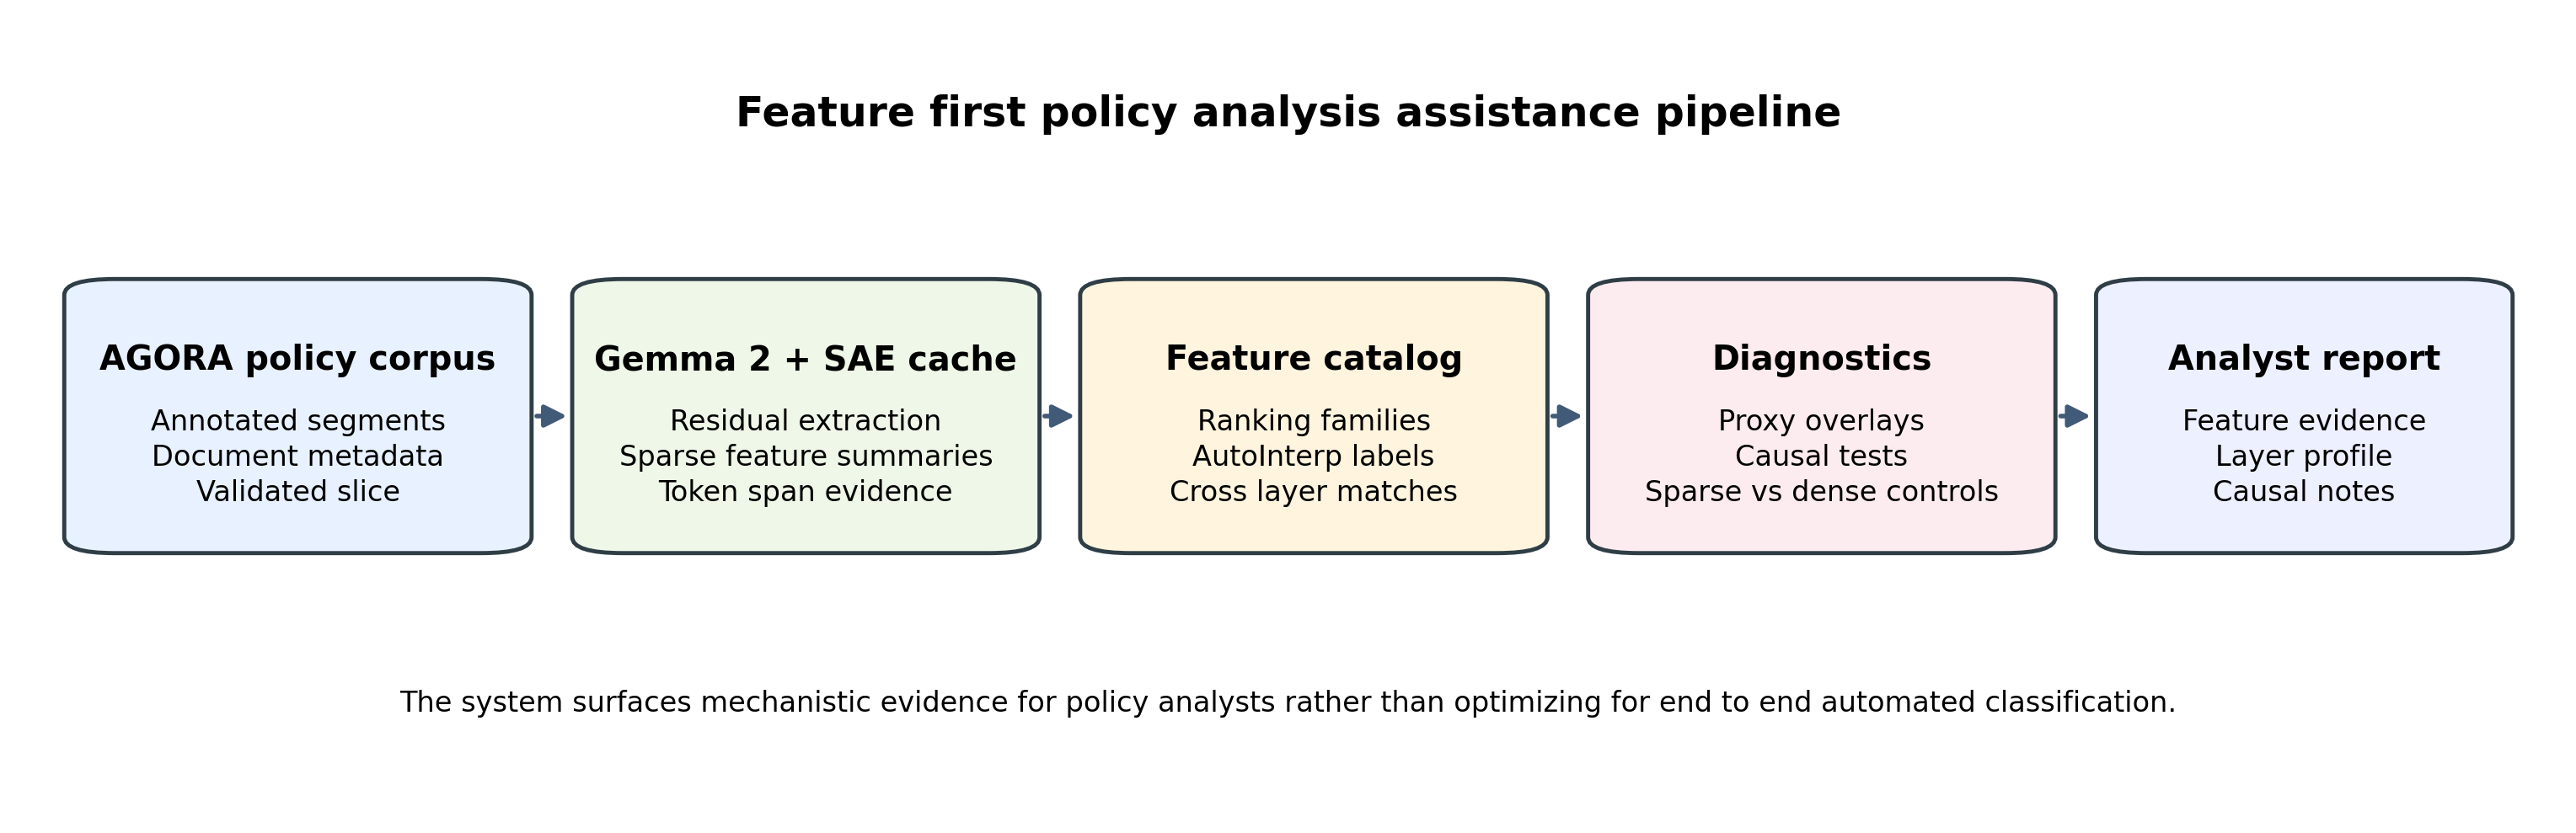
\includegraphics[width=0.95\textwidth]{figures/system_overview_tool.png}
    \caption{System overview of the audit stack. AGORA passages are processed with Gemma 2 2B and Gemma Scope sparse autoencoders, producing feature summaries, feature catalogs, AutoInterp labels, cross-layer overlap statistics, proxy overlays, and causal diagnostics. New statutory passages are then scored against the same catalog to produce audit records rather than end-to-end classifications.}
    \label{fig:system-overview}
\end{figure*}

\Cref{fig:system-overview} shows the full stack. The corpus side constructs a reusable sparse cache from AGORA. The feature side builds ranked catalogs, attaches automated interpretations, and computes post hoc overlays and causal summaries. The report side takes a new passage and returns activated features, evidence spans, proxy overlays, and causal notes. The result is an evidence store for auditing rather than a black-box predictor.

\section{Feature-First Audit Engine}

\paragraph{Data and model setup.}
We work with 2,891 AGORA segments from 331 documents after filtering for annotated, operative, and AI-related material \cite{arnold2024agora}. The working splits are 1,830 train, 317 dev, 375 test, and a separate validated slice of 369 segments. We use Gemma 2 2B with Gemma Scope 16k residual stream sparse autoencoders at layers 12, 16, 20, and 24 \cite{gemma2024, lieberum2024gemmascope}. All reported main-text results fit the medium-local constraint of a single RTX 3090 class machine.

\begin{table}[t]
    \centering
    \caption{Dataset summary with split sizes and proxy counts.}
    \label{tab:dataset-summary}
    \scriptsize
    \begin{tabular}{lrrrr}
        \toprule
        Statistic & Train & Dev & Test & Validated \\
        \midrule
        Segments & 1830 & 317 & 375 & 369 \\
        Documents & 187 & 44 & 44 & 56 \\
        Privacy & 170 & 27 & 32 & 46 \\
        Bias & 148 & 27 & 26 & 45 \\
        Discrimination & 112 & 27 & 25 & 34 \\
        Transparency & 185 & 35 & 28 & 66 \\
        Rights violation & 242 & 26 & 29 & 62 \\
        Interpretability & 40 & 7 & 10 & 15 \\
        \bottomrule
    \end{tabular}
\end{table}

\paragraph{Feature catalog and ranking families.}
The pipeline is feature-first rather than module-first. For every feature we store activation count, activation frequency, mean positive activation, tail activation statistics, document frequency, and token-peak summaries. These support three ranking families: \emph{global dominance}, \emph{policy specific}, and \emph{layer unique}. The resulting catalog stores top activating spans, exemplars, logit attribution summaries, decoder vectors, and post hoc proxy overlaps.

\paragraph{AutoInterp, cross-layer structure, and overlays.}
Candidate features from the policy-specific and layer-unique families are labeled with an AutoInterp loop using top contexts and contrastive low-activation snippets \cite{bills2023neurons, paulo2025autointerp, eleuther2024autointerp}. Importantly, proxy overlays are added only after discovery. Privacy, bias, discrimination, transparency, rights-violation, and interpretability are annotations on the catalog rather than search criteria. Cross-layer overlap then lets us ask whether policy-relevant sparse features persist, specialize, or disappear as the model processes text.

\paragraph{Why feature-first.}
This pivot is empirically motivated. On the full layer-24 run, sparse module probes reach only 0.460 privacy test AUC and 0.474 bias test AUC, while individual sparse feature probes reach 0.651 and 0.646. The average individual-minus-module gap is therefore 0.145. We retain module analysis as secondary evidence, but the main audit interface is the feature catalog because it preserves more mechanistic signal.

\section{Audit Outputs on Real Statutory Text}

\begin{figure*}[t]
    \centering
    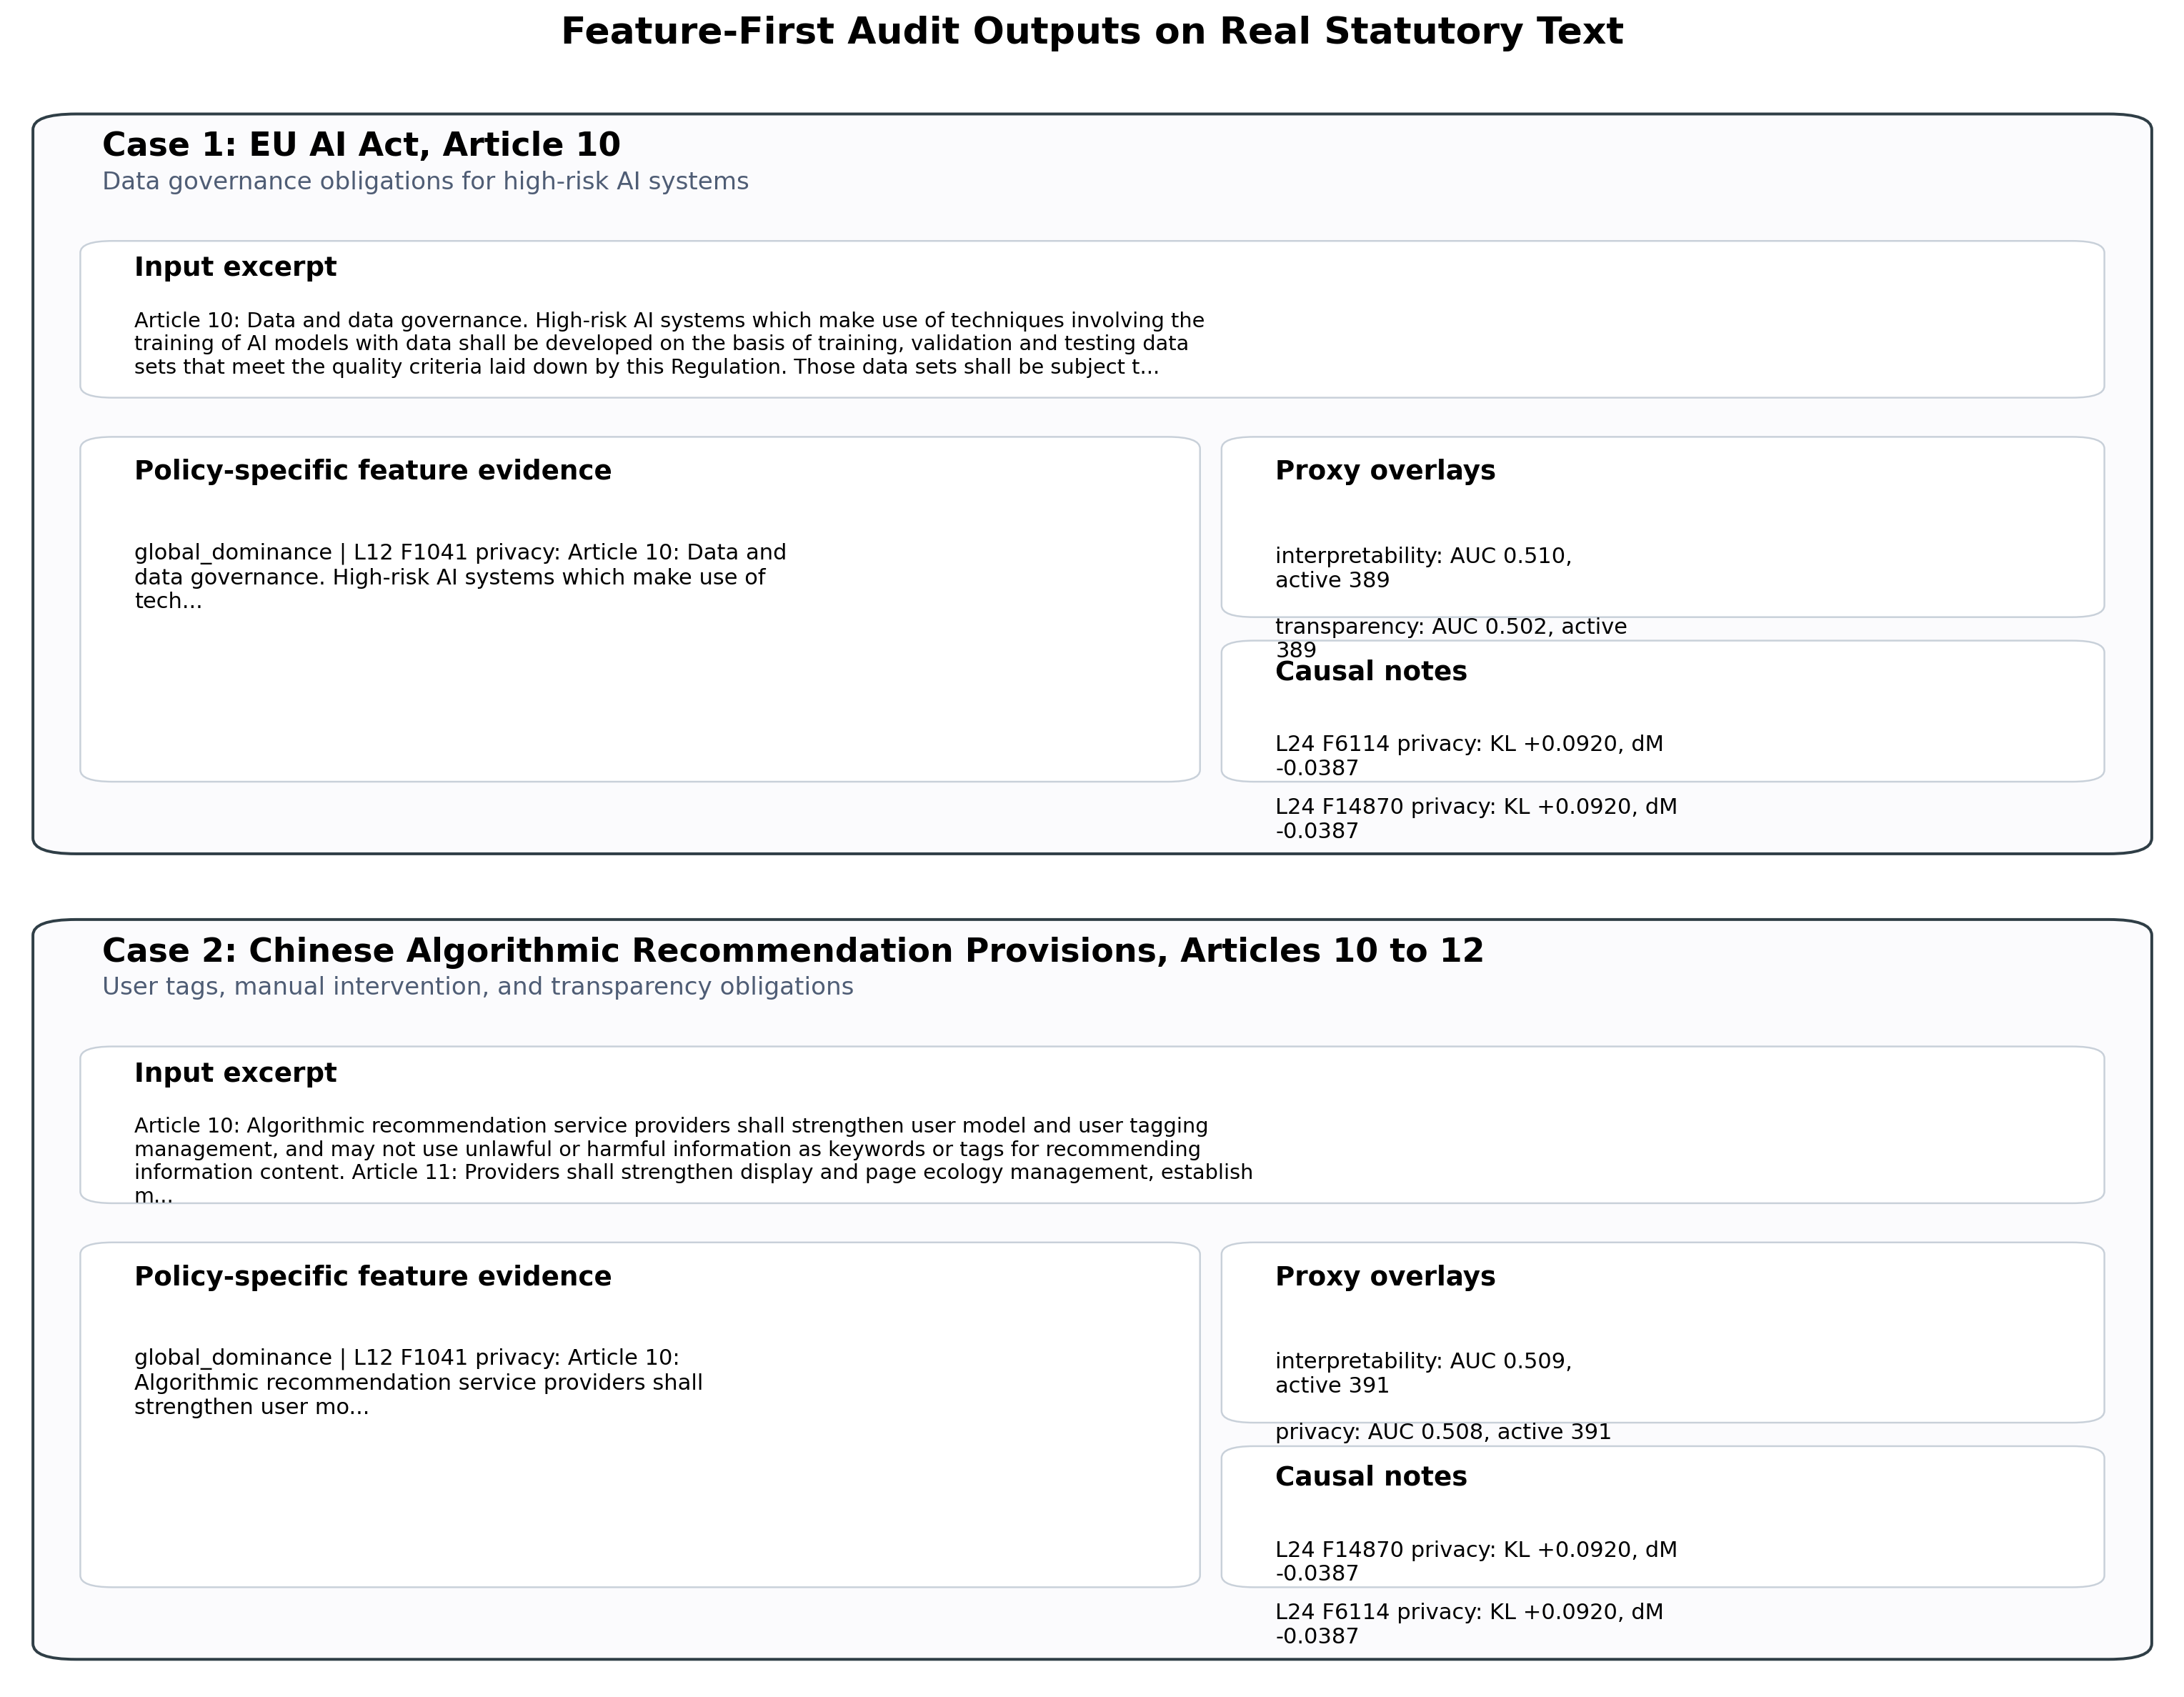
\includegraphics[width=0.96\textwidth]{figures/workflow_case_reports.png}
    \caption{Example audit outputs on real statutory text. The first panel uses Article 10 of the EU AI Act. The second uses Articles 10 to 12 of the Chinese Algorithmic Recommendation Management Provisions. Each report foregrounds policy-specific feature evidence, one global anchor, post hoc proxy overlays, and causal notes. The screenshot is an audit-output demo, not the primary evidence of usefulness.}
    \label{fig:workflow-cases}
\end{figure*}

We use real law excerpts in AGORA rather than synthetic prompts. The first case is Article 10 of the EU AI Act on data and data governance for high-risk AI systems. The second is Articles 10 to 12 of the Chinese \emph{Internet Information Service Algorithmic Recommendation Management Provisions} on user tagging, manual intervention, and transparency. These cases are difficult because both mix multiple governance themes and both trigger generic legal structure features. \Cref{fig:workflow-cases} therefore serves as a demonstration of the audit record rather than as the primary evaluation.

The key lesson from these cases is also a negative one. If the auditor looks only at the strongest overall features, the two laws appear overly similar because ubiquitous features dominate. The policy-specific view partially resolves this problem by surfacing features tied to high-risk governance, user-tagging procedures, or procedural transparency. This observation motivates the main compute-only audit evaluations below.

\begin{figure*}[t]
    \centering
    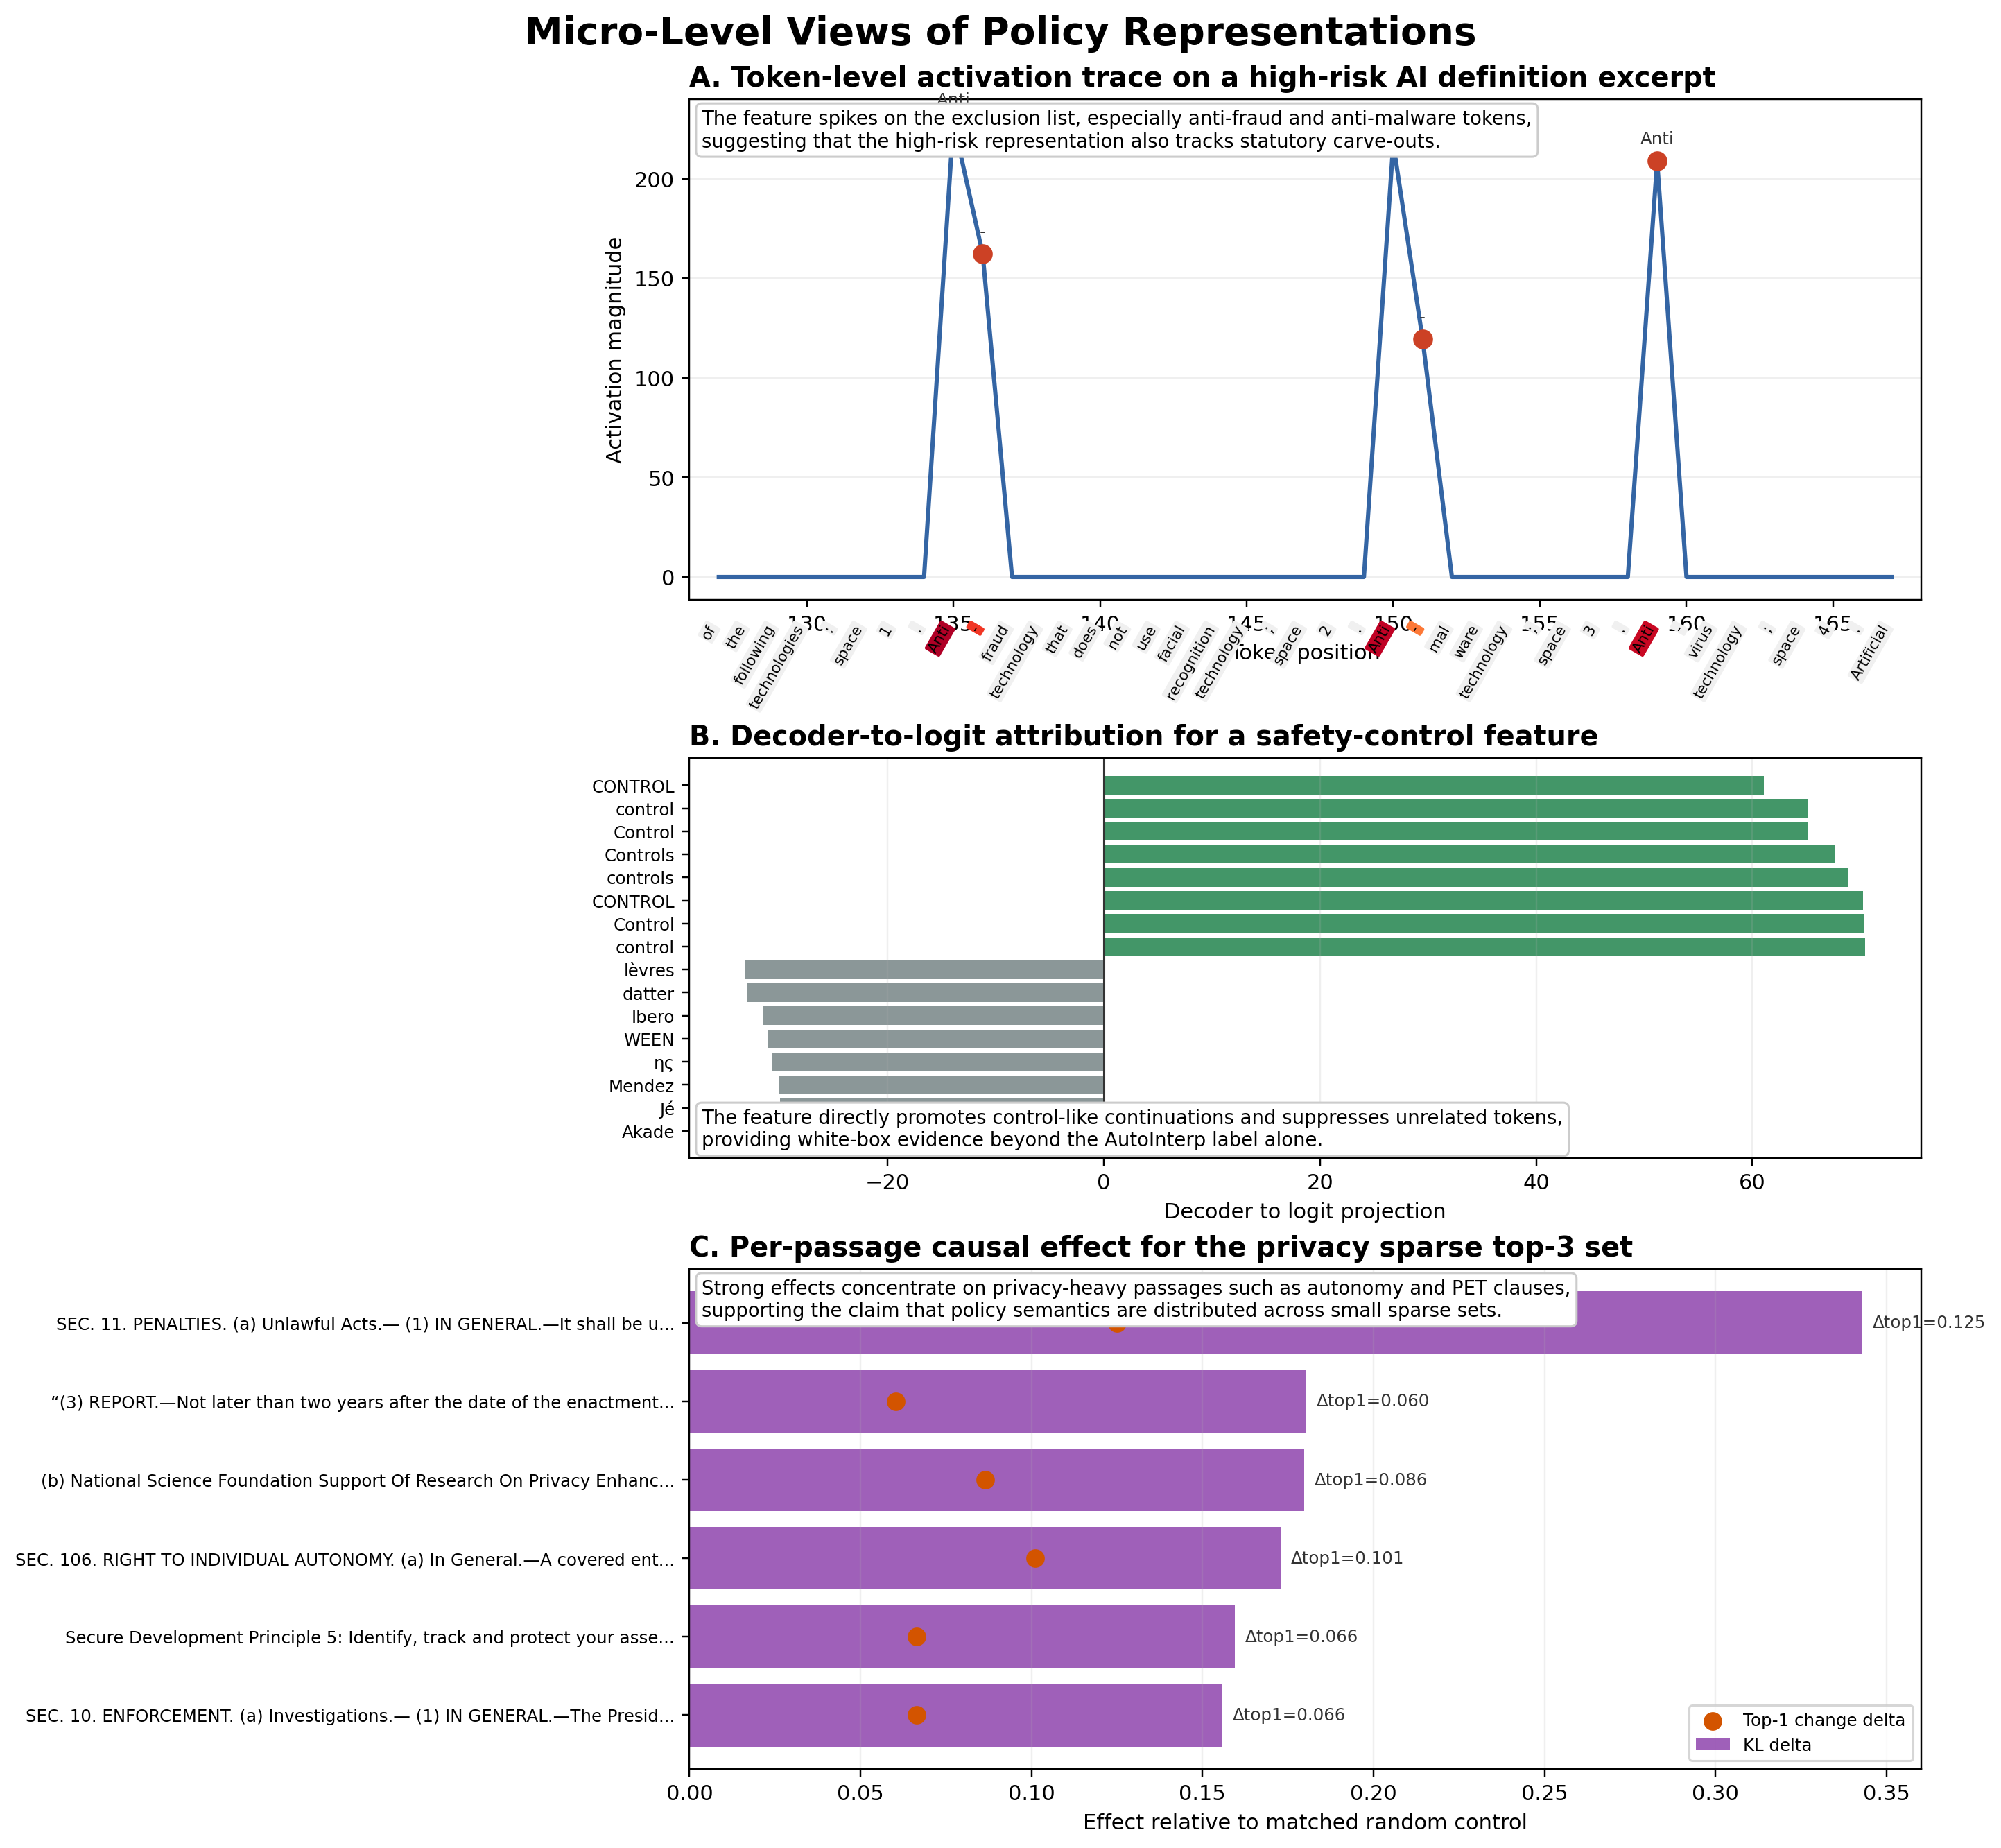
\includegraphics[width=0.95\textwidth]{figures/mech_interp_micro_views.png}
    \caption{Micro-level views of the audit surface. Panel A shows a token-level activation trace for the layer-20 \emph{High Risk Decision Systems} feature on a statutory definition excerpt, where the strongest spikes fall on anti-fraud and anti-malware exclusion tokens inside a high-risk carve-out list. Panel B projects the layer-12 \emph{Control Measures Safety} feature through the unembedding matrix and shows that it directly promotes control-like continuations. Panel C visualizes per-passage causal effects for the privacy sparse top-3 set, showing that proxy-free perturbation concentrates on a small number of privacy-heavy passages rather than spreading uniformly across the evaluation split.}
    \label{fig:micro-mech}
\end{figure*}

Macro-level summaries are only part of the story. \Cref{fig:micro-mech} adds the kind of micro-level evidence commonly expected in mechanistic interpretability work. The token trace shows that a layer-20 feature associated with high-risk decision systems also fires on statutory exclusion language, suggesting that the representation bundles the main concept with its legal carve-outs. The decoder-to-logit view shows that a layer-12 control feature directly pushes control-related continuations, providing white-box evidence beyond the AutoInterp label alone. The per-passage intervention panel then closes the loop by showing that the strongest privacy sparse set effects concentrate on a handful of privacy-heavy clauses rather than on every policy passage equally.

\section{Empirical Evaluation}

\subsection{Audit coverage}

\begin{figure*}[t]
    \centering
    
\includegraphics[width=0.94\textwidth]{figures/policy_feature_map.png}
    \caption{Policy feature map as an audit surface across layers 12, 16, 20, and 24. Marker color indicates AutoInterp faithfulness, shape indicates ranking family, and border color indicates the strongest post hoc proxy overlay. Star markers denote features previously tested in the causal pipeline. The map shows policy-relevant sparse features across layers, with the clearest policy-specific concentration around layer 20.}
    \label{fig:policy-feature-map}
\end{figure*}

The feature map in \cref{fig:policy-feature-map} is the main audit-coverage result. We obtain 68 scored AutoInterp features across four sampled layers. Mean held-out faithfulness is 0.510 at layers 12 and 20, 0.490 at layer 16, and 0.412 at layer 24. High-faithfulness counts above the 0.667 threshold are 1, 0, 2, and 0 respectively. The best-scoring policy-specific features appear at layer 20, including \emph{High Risk Decision Systems} and \emph{Microelectronics}. Cross-layer overlap is local rather than global: policy-specific set overlap is 0.282 for layers 12 and 16, 0.190 for layers 20 and 24, and near zero for distant pairs such as 12 and 24. Together with the micro-level traces in \cref{fig:micro-mech}, the audit surface supports a staged representation story rather than a single terminal policy layer.

\begin{table*}[t]
    \centering
    \caption{Representative curated features from the audit catalog. Contrastive accuracy measures whether the explanation scores held-out positives above matched negatives.}
    \label{tab:curated-features}
    \small
    \begin{tabular}{rllrrr}
        \toprule
        Layer & Feature name & Family & Best proxy & Faithfulness & Contrastive accuracy \\
        \midrule
        12 & Control Measures Safety & layer unique & privacy & 0.833 & 1.000 \\
        12 & Catastrophic Outcomes Outcomes Would & policy specific & bias & 0.667 & 0.667 \\
        16 & Reasoning & layer unique & interpretability & 0.667 & 0.667 \\
        16 & Deadlines Timeframes Related Implementation & policy specific & interpretability & 0.667 & 0.667 \\
        20 & High Risk Decision Systems & policy specific & discrimination & 0.833 & 0.889 \\
        20 & Microelectronics & policy specific & bias & 0.833 & 0.944 \\
        24 & Consequential Decision Impact Consumers & policy specific & bias & 0.667 & 1.000 \\
        24 & Development Systems National Security & policy specific & interpretability & 0.500 & 0.500 \\
        \bottomrule
    \end{tabular}
\end{table*}

\subsection{Audit discriminativeness}

\begin{figure*}[t]
    \centering
    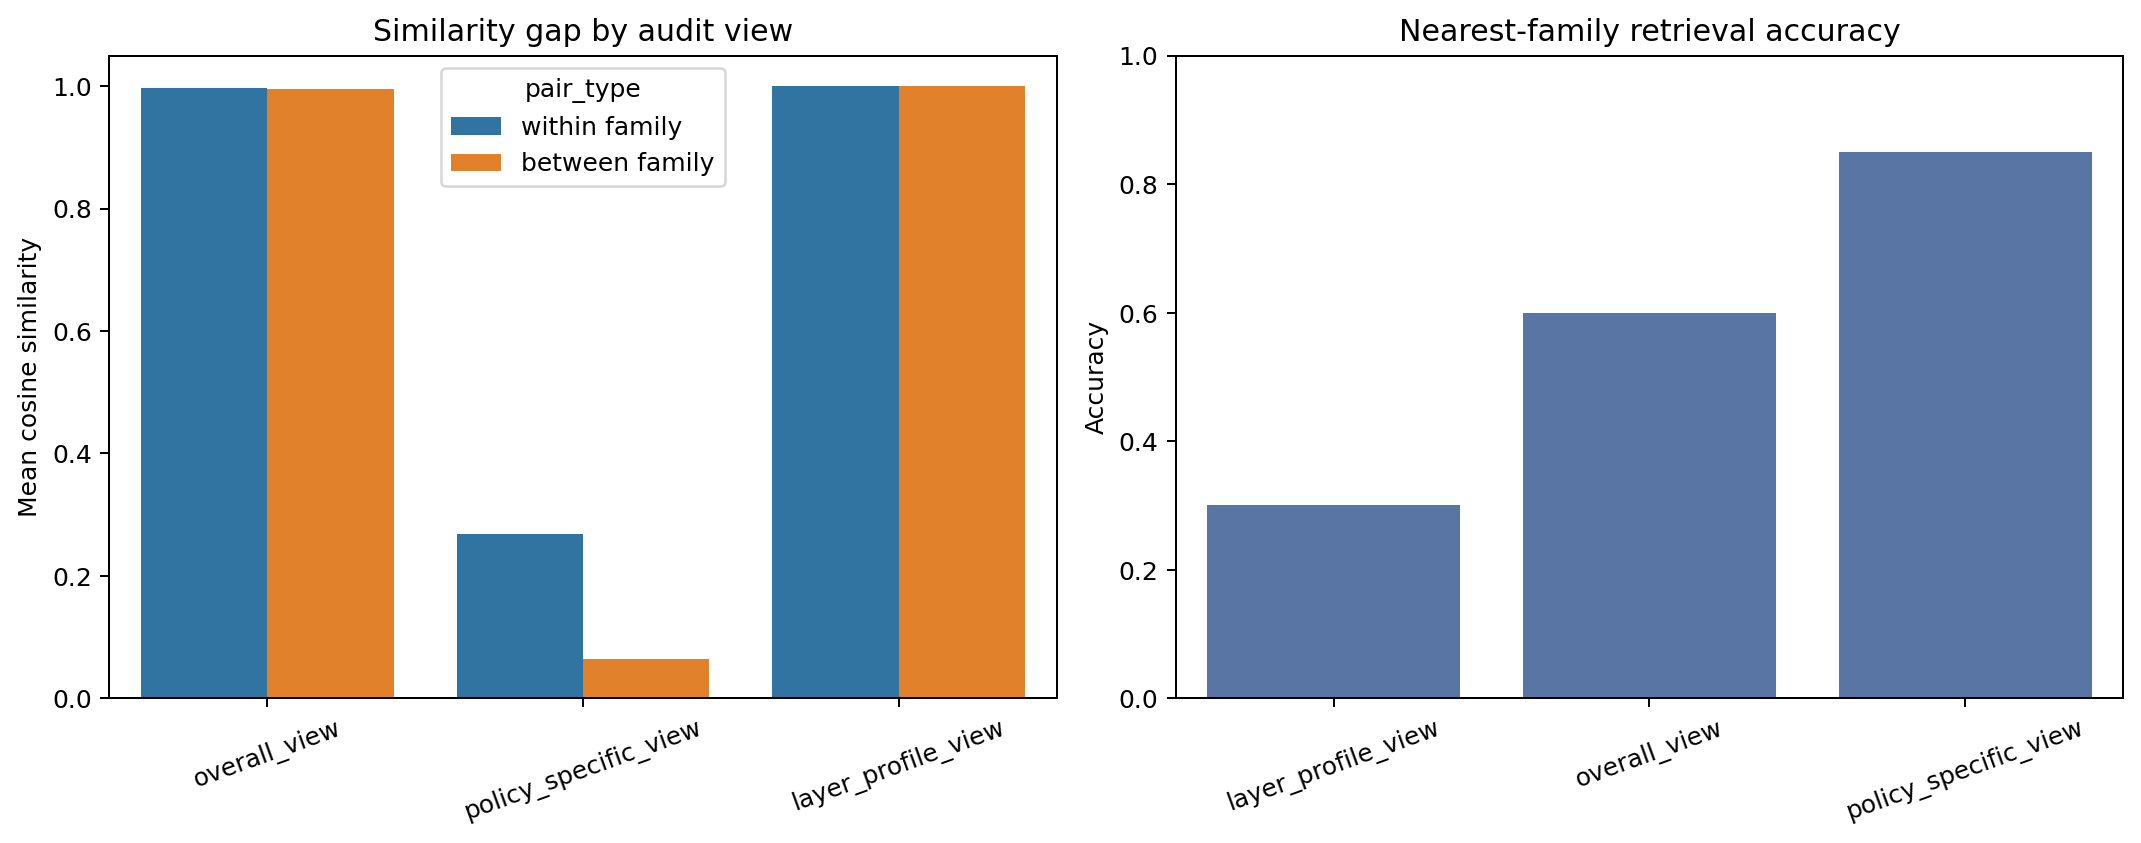
\includegraphics[width=0.92\textwidth]{figures/audit_discriminativeness.png}
    \caption{Compute-only audit discriminativeness. The left panel compares within-family and between-family cosine similarity for three audit views. The right panel shows nearest-family retrieval accuracy. The policy-specific view separates held-out regulatory families much better than the overall sparse view or the layer-profile-only view.}
    \label{fig:audit-discriminativeness}
\end{figure*}

The main utility result is compute-only. We construct 20 held-out statutory excerpts from four law families: EU high-risk AI governance, Chinese algorithmic recommendation rules, privacy and data-protection regulation, and governance principles or safety frameworks. We then ask whether different audit views can recover law-family structure. The answer is yes, but only for the policy-specific view.

\begin{table}[t]
    \centering
    \caption{Audit discriminativeness across 20 held-out statutory excerpts.}
    \label{tab:audit-discriminativeness}
    \scriptsize
    \begin{tabular}{lrrr}
        \toprule
        View & Cosine gap & Jaccard gap & Retrieval \\
        \midrule
        Layer profile only & 0.000 & n/a & 0.30 \\
        Overall sparse view & 0.002 & 0.035 & 0.60 \\
        Policy-specific view & 0.204 & 0.050 & 0.85 \\
        \bottomrule
    \end{tabular}
\end{table}

As shown in \cref{fig:audit-discriminativeness,tab:audit-discriminativeness}, the overall sparse view is dominated by generic features and therefore almost collapses within-family and between-family similarity. Its cosine gap is only 0.0018 and retrieval accuracy is 0.60. In contrast, the policy-specific view achieves a cosine gap of 0.204 and nearest-family retrieval accuracy of 0.85. This is the clearest evidence that the audit stack surfaces regime-specific internal evidence rather than merely reproducing generic legal structure.

\subsection{Causal diagnostics and failure transparency}

We evaluate report robustness by perturbing the same 20 excerpts with heading removal, lexical anchor masking, and sentence compression. Policy-specific feature sets remain relatively stable under heading removal and lexical masking, with mean policy-specific Jaccard 0.925 and 0.862 respectively. Sentence compression is harsher but still leaves a mean policy-specific Jaccard of 0.748, proxy-rank Spearman 0.986, and layer-profile cosine essentially 1.0. This robustness pattern supports the claim that the audit stack captures more than exact lexical matching, even though some signals remain brittle.

AutoInterp validation is mixed but usable. Layer 20 has the highest mean contrastive accuracy at 0.598 and shares the highest mean faithfulness with layer 12 at 0.510. Mean lexicality penalties remain moderate, between 0.49 and 0.59, which suggests that many explanations are not pure token copies but still overlap substantially with their top spans. We therefore treat AutoInterp labels as ranked hypotheses rather than as definitive semantic ground truth.

\begin{figure*}[t]
    \centering
    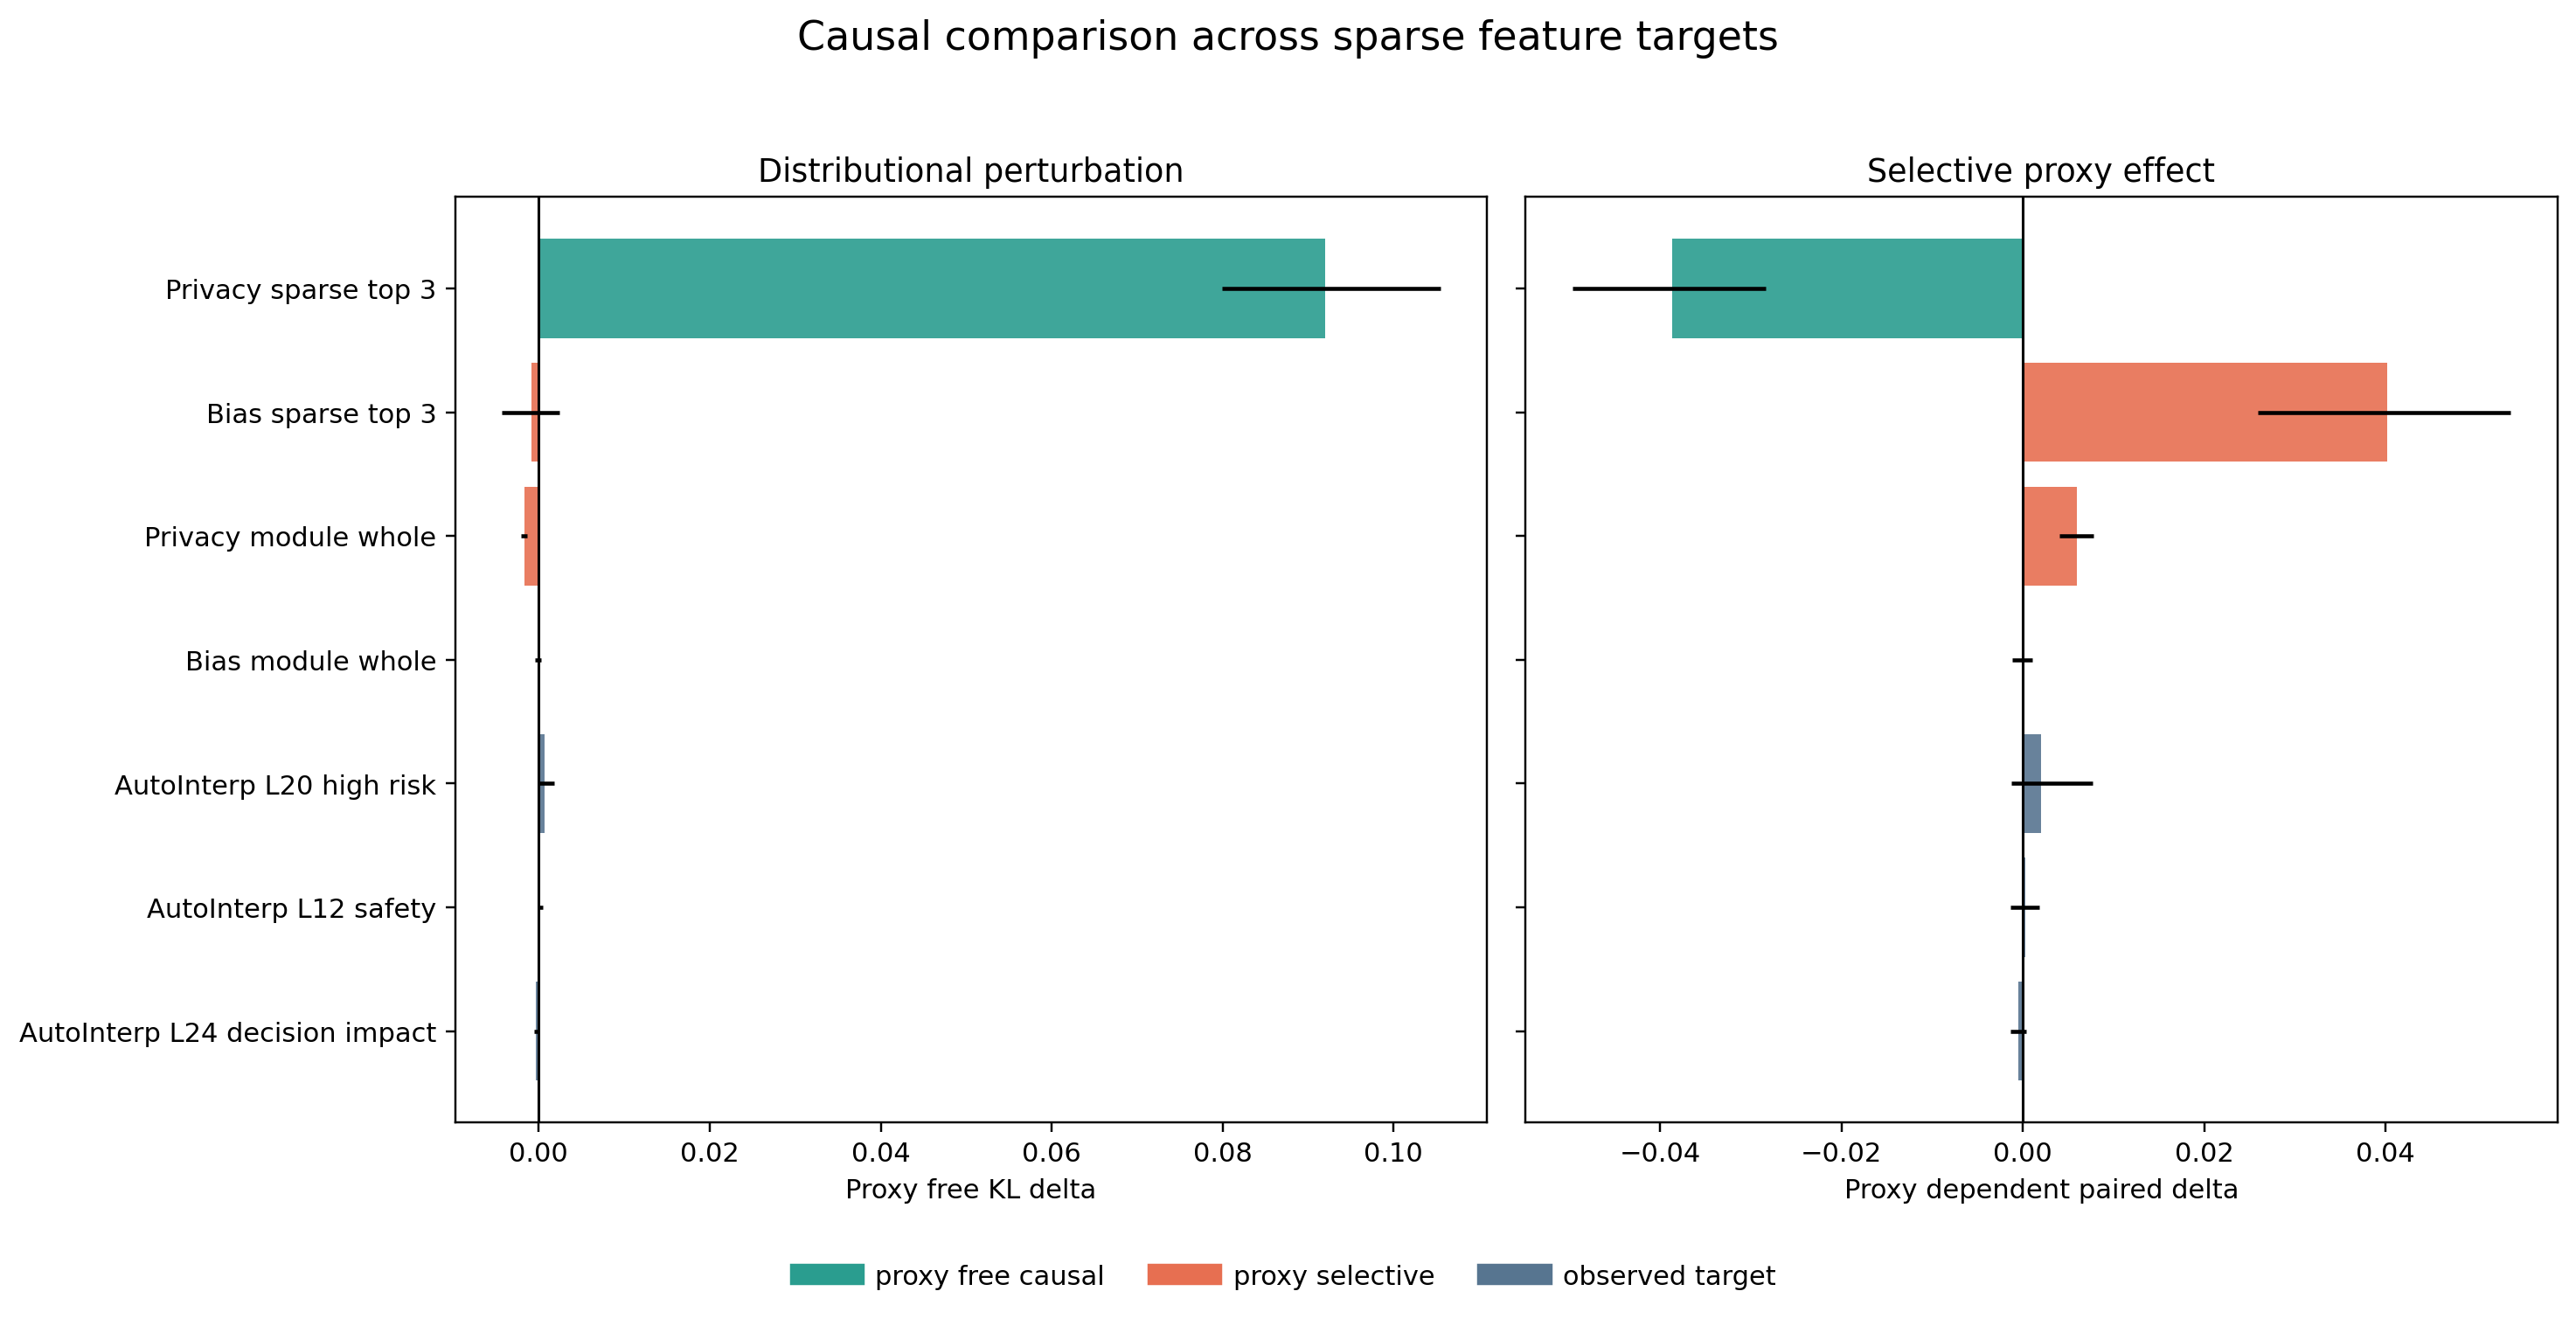
\includegraphics[width=0.95\textwidth]{figures/causal_comparison_summary.png}
    \caption{Causal comparison across sparse targets. The left panel shows proxy-free KL divergence deltas relative to matched random controls, and the right panel shows proxy-dependent paired deltas. The strongest proxy-free effect still comes from the privacy sparse top-3 set, not from any single AutoInterp feature.}
    \label{fig:causal-comparison}
\end{figure*}

The causal section reinforces the same failure-transparent story. Existing interventions show that single AutoInterp features are usually weak control points, while small sparse sets can be much stronger. The privacy individual top-3 set yields KL divergence delta $+0.0920$ and perplexity shift delta $+1.403$, far above any tested single feature. The best single feature, layer-20 \emph{High Risk Decision Systems}, has only KL delta $+0.0006$ and paired delta $+0.0020$. Module-wide interventions are weaker still. The micro-level view in \cref{fig:micro-mech} makes the same point more concretely: causal influence is real, but it is concentrated in sparse bundles and on a limited subset of passages.

\begin{table*}[t]
    \centering
    \caption{Causal comparison between legacy sparse targets and single AutoInterp features. Positive paired delta indicates stronger proxy-selective effect than matched random controls. Positive KL delta indicates stronger proxy-free perturbation than matched random controls.}
    \label{tab:causal-summary}
    \small
    \begin{tabular}{llrrlll}
        \toprule
        Target & Kind & Layer & Proxy & Paired delta & KL delta & Badge \\
        \midrule
        Privacy sparse top 3 & feature topk & 24 & privacy & $-0.0387$ & $+0.0920$ & proxy-free causal \\
        Bias sparse top 3 & feature topk & 24 & bias & $+0.0402$ & $-0.0008$ & proxy-selective \\
        Privacy module whole & module whole & 24 & privacy & $+0.0060$ & $-0.0017$ & proxy-selective \\
        Bias module whole & module whole & 24 & bias & $-0.0001$ & $-0.0002$ & observed target \\
        AutoInterp L20 high risk & single feature & 20 & discrimination & $+0.0020$ & $+0.0006$ & observed target \\
        AutoInterp L12 safety & single feature & 12 & privacy & $+0.0002$ & $+0.0002$ & observed target \\
        AutoInterp L24 decision impact & single feature & 24 & bias & $-0.0005$ & $-0.0003$ & observed target \\
        \bottomrule
    \end{tabular}
\end{table*}

Failure transparency turns these negatives into quantitative audit findings. Among top overall features, 96.7\% are effectively ubiquitous with activation frequency at or near one. The mean individual-feature minus module-probe test-AUC gap is 0.145. Among top policy-specific features, 80\% have shallow best-versus-runner-up proxy margins. Among tested single AutoInterp features, 75\% have near-zero proxy-free and proxy-dependent effects. These are precisely the kinds of observations that black-box audits miss.

\section{Discussion and Limitations}

The central takeaway is not that policy-relevant behavior collapses to a small set of monosemantic sparse features. The stronger claim is narrower and, we think, more useful: a feature-first audit stack can expose nontrivial internal structure, distinguish regulatory regimes better than generic sparse summaries, and surface its own failure modes instead of hiding them. The added micro-level figures matter here because they show that the system is not only producing aggregate tables. It can also reveal which tokens trigger a feature, which continuations a feature promotes, and which passages are most affected by sparse interventions.

Several limitations matter. First, this is an offline audit stack rather than an interactive production system. Second, AutoInterp labels remain hypotheses, supported by held-out faithfulness and contrastive tests but not elevated to ground-truth semantics. Third, single-feature control is usually weak, and a full layer-wise top-3 and top-5 concentration sweep remained outside the medium-local compute budget of this submission. Fourth, proxy overlays are annotations rather than discovery criteria, which prevents circularity but also limits how strongly they should be interpreted. Finally, policy-relevant auditing does not imply legal compliance auditing or policy correctness.

\section{Conclusion}

We introduced a feature-first mechanistic auditing pipeline for policy-relevant model behavior. The system turns AGORA and Gemma Scope into a reusable white-box audit surface with sparse features, activating spans, AutoInterp labels, proxy overlays, and causal notes. On held-out statutory excerpts, the policy-specific view separates regulatory regimes much better than overall sparse summaries, while robustness and failure-transparency analyses show both what the pipeline captures and where it breaks. The empirical picture is mixed by design: policy-relevant sparse features are visible and useful for auditing, but the strongest causal effects remain distributed rather than concentrated in single features. We view that negative result as part of the contribution.

\section*{Impact Statement}

This paper studies how to inspect model behavior on policy-relevant text. The potential benefit is better white-box auditing of internal model behavior on governance and statutory material. The potential risk is over-interpreting sparse features or automated labels as legal conclusions. We therefore frame the system as a mechanistic auditing stack for model behavior, not as a compliance tool or substitute for legal judgment.

\bibliography{policy_feature_map_refs}
\bibliographystyle{icml2026}

\newpage
\appendix
\onecolumn

\section{Appendix A: Feature-First Pivot Rationale}

The feature-first pivot was driven by full-run evidence rather than by aesthetic preference. On layer 24, sparse module probes achieved privacy and bias test AUCs of 0.460 and 0.474, while sparse individual-feature probes reached 0.651 and 0.646. Pilot-to-full module overlap was also weak. These results justify treating modules as secondary analysis and foregrounding feature catalogs in the main paper.

\section{Appendix B: Audit Discriminativeness Details}

The audit discriminativeness benchmark contains 20 held-out excerpts from four families: EU high-risk AI governance, Chinese algorithmic recommendation rules, privacy and data-protection regulation, and governance principles or safety frameworks. Each family contributes five excerpts chosen under a fixed split-priority rule. We compare three views: overall sparse features, policy-specific sparse features, and layer profiles. The policy-specific view is the only one that clearly separates families in both cosine similarity and nearest-family retrieval.

\begin{figure}[h]
    \centering
    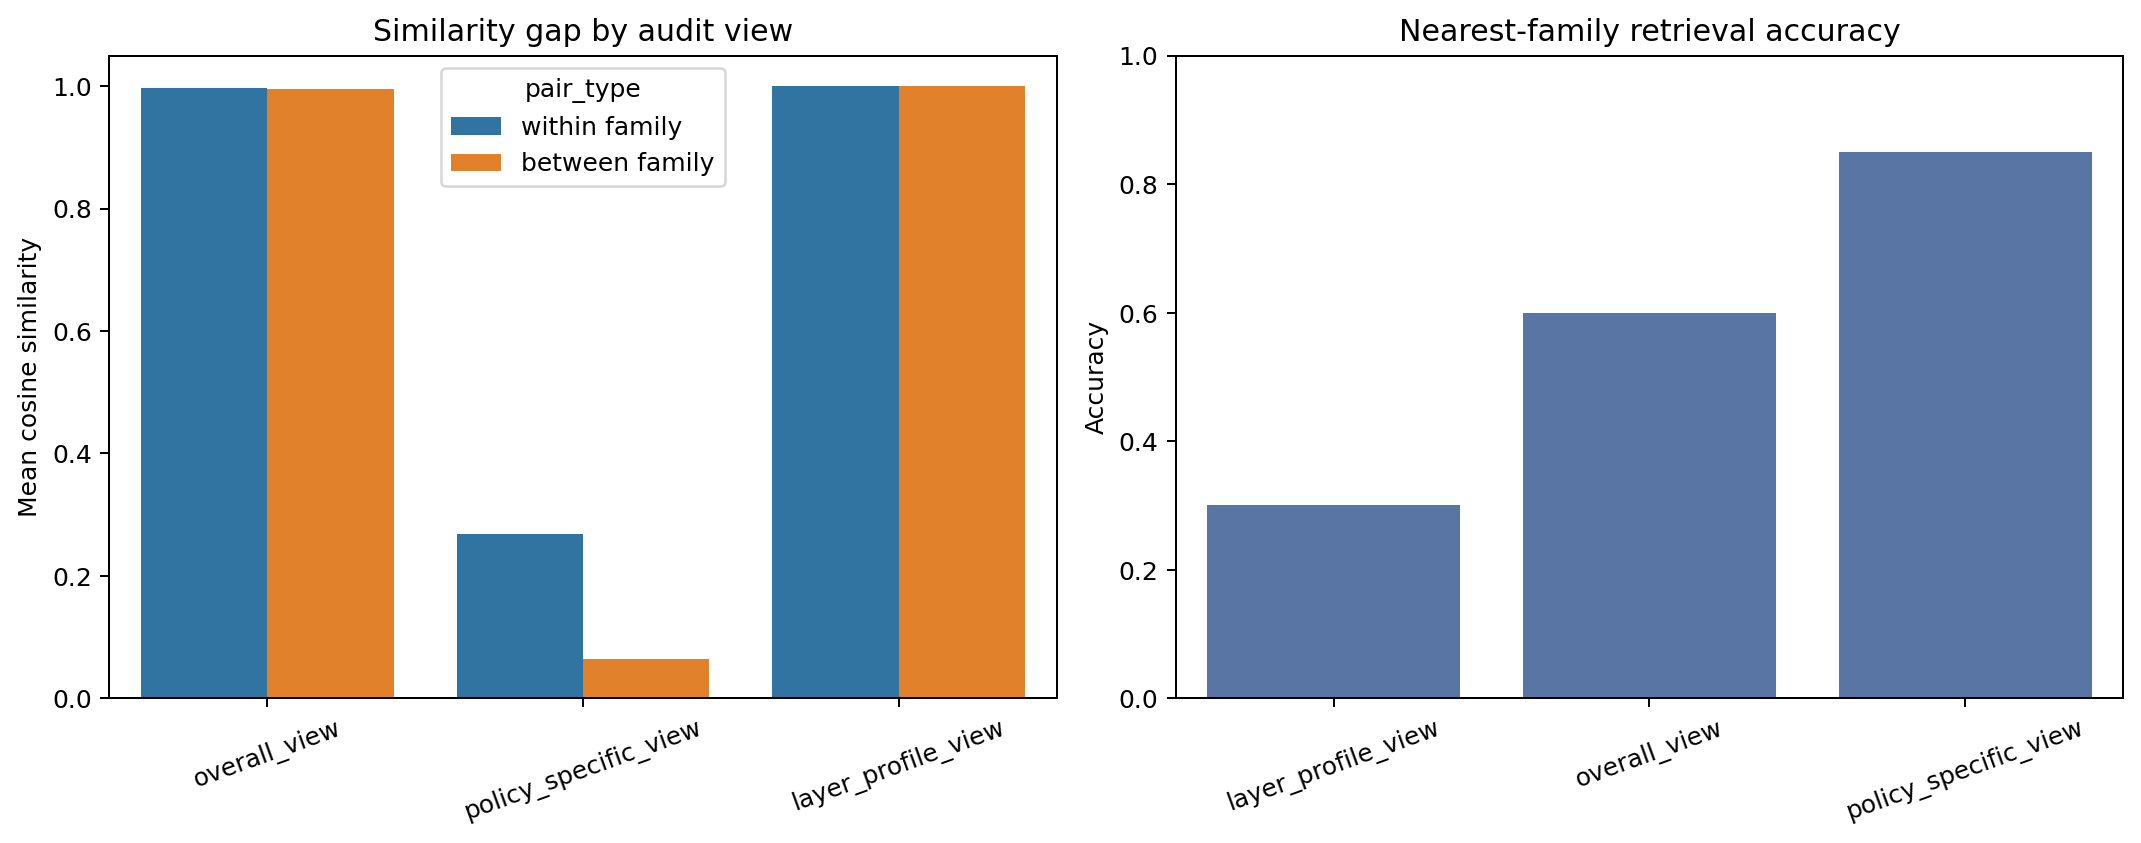
\includegraphics[width=\textwidth]{figures/audit_discriminativeness.png}
    \caption{Audit discriminativeness in the appendix for direct reference.}
    \label{fig:appendix-audit-discriminativeness}
\end{figure}

\section{Appendix C: Report Robustness}

We test robustness under heading removal, lexical anchor masking, and sentence compression. Overall features remain extremely stable because generic features dominate them. Policy-specific features are more informative and somewhat less stable, which is the expected trade-off for an audit view intended to distinguish regulatory regimes.

\begin{figure}[h]
    \centering
    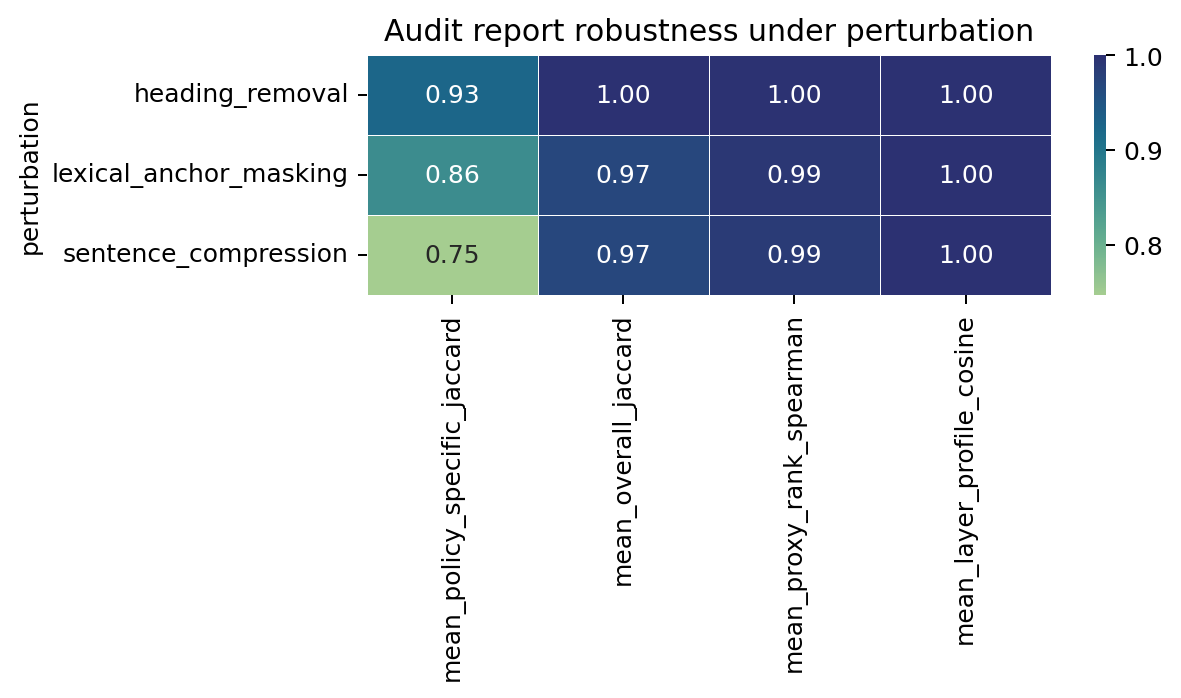
\includegraphics[width=\textwidth]{figures/audit_report_robustness.png}
    \caption{Report robustness under mild textual perturbations.}
    \label{fig:appendix-robustness}
\end{figure}

\section{Appendix D: AutoInterp Scoring Protocol}

AutoInterp uses top contexts, contrastive low-activation examples, and boundary prompts to generate feature descriptions. We score these descriptions on held-out positives and negatives, then compute a contrastive accuracy and a lexicality penalty. The main text reports layer-level aggregates: mean faithfulness, count above a high-faithfulness threshold, mean contrastive accuracy, and mean lexicality penalty.

\section{Appendix E: Full Causal Diagnostics}

The main text reports legacy sparse top-3 targets, module-wide interventions, and single AutoInterp features. Within the medium-local compute budget, these already establish the most important pattern: small sparse sets can produce stronger perturbations than single features, while single-feature causal control is usually weak. A larger layer-wise top-3 and top-5 sweep remains future work.

\section{Appendix F: Negative Result Transparency}

We explicitly surface negative results because they matter for audit credibility.

\begin{figure}[h]
    \centering
    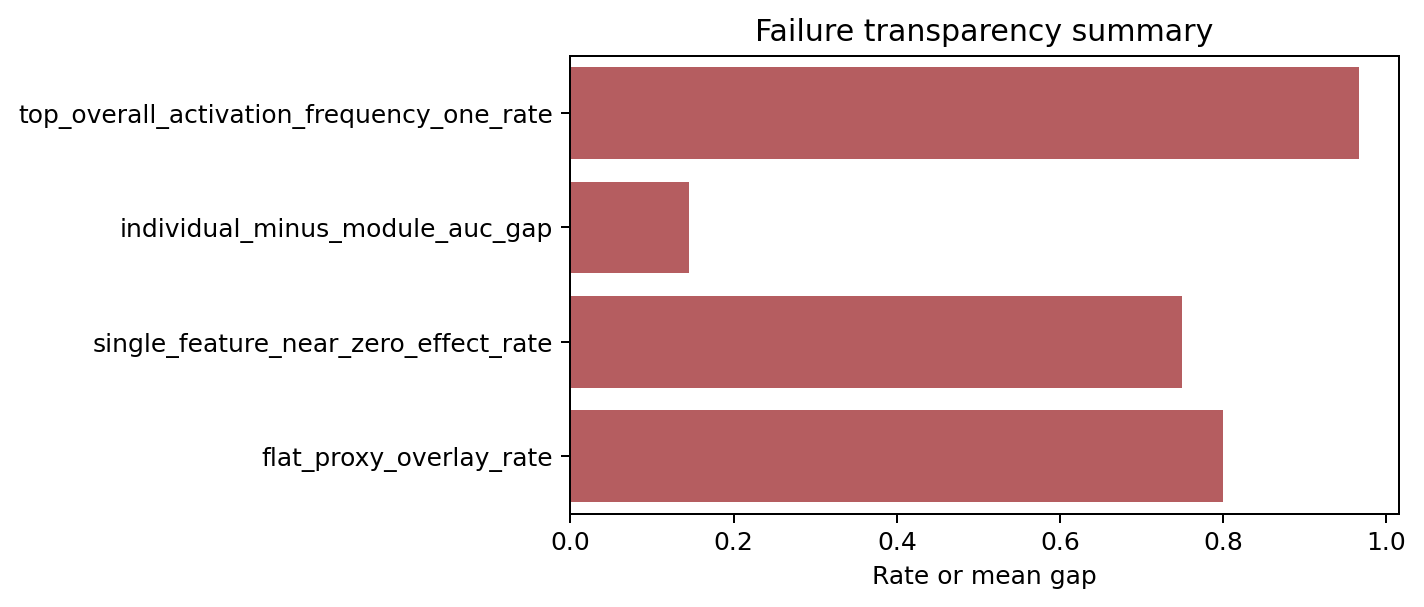
\includegraphics[width=0.8\textwidth]{figures/failure_transparency.png}
    \caption{Failure-transparency summary. Ubiquitous global features, flat proxy overlays, weak single-feature effects, and the module-versus-individual gap are central audit findings rather than incidental artifacts.}
    \label{fig:appendix-failure}
\end{figure}

\begin{table}[h]
    \centering
    \caption{Layer 24 baseline comparison. Dense and sentence-level baselines outperform sparse probes on prediction, while sparse individual features still outperform sparse modules by a wide margin.}
    \label{tab:baseline-appendix}
    \small
    \begin{tabular}{llrr}
        \toprule
        Proxy & Method & Dev AUC & Test AUC \\
        \midrule
        Privacy & Dense residual LR & 0.865 & 0.823 \\
        Privacy & Sentence embedding LR & 0.884 & 0.810 \\
        Privacy & Sparse individual feature probe & 0.725 & 0.651 \\
        Privacy & Sparse module probe & 0.466 & 0.460 \\
        Bias & Dense residual LR & 0.915 & 0.880 \\
        Bias & Sentence embedding LR & 0.816 & 0.828 \\
        Bias & Sparse individual feature probe & 0.672 & 0.646 \\
        Bias & Sparse module probe & 0.509 & 0.474 \\
        \bottomrule
    \end{tabular}
\end{table}

\section{Appendix G: Reproducibility and Compute}

All main results use Gemma 2 2B with Gemma Scope 16k sparse autoencoders on sampled layers 12, 16, 20, and 24. Artifact generation, feature catalogs, AutoInterp labels, audit discriminativeness summaries, robustness summaries, and paper figures are cached under the experiment root. The medium-local constraint of a single RTX 3090 class machine shaped which intervention sweeps were feasible within this submission cycle.

\end{document}
